% Yachay-Physics School-Template, 2025/04/02
% Copyright (C) 2025-2035 Mario D. Andrango Torres (and_damian@outlook.com)
%
% This work may be distributed and/or modified under the conditions of the
% LaTeX Project Public License, either version 1.3 of this license or (at your
% option) any later version.
% The latest version of this license is in
% https://www.latex-project.org/


\documentclass[
  aspectratio = 169,% Ratio de aspecto: 43 (4:3), 169 (16:9), etc.
  10pt,% Tamaño de la fuente
  t,% alinea el contenido al top (arriba) del cuadro de cada diapositiva.
  onlytextwidth,% restringe el contenido a la anchura del texto ()
  compress,% Comprime la barra de navegación.
  %handout,% Genera una versión sin efectos de transición ni overlays (útil para imprimir o compartir) comentar cuando se desea efectos de transición ordenada. 
  xcolor = table,% Usamos el paquete colortb, para dar color a las tablas.
  english % Idioma secundario(penúltimo)
  spanish,% Idioma principal
]{beamer}

\usepackage[%% Opções (^ = padrão; ¹ = Apresentação; ² = Artigo):
%   Layout    = Beamer,%% Leiaute (blocos): TCB (tcolorbox) (^) ou Beamer
%   Font      = Arial,%% Fonte principal: Arial, Calibri, Times ou LaTeX(*) (^)
%   LinkColor = ,%% Cor (Modelo HTML) hyperlink (azul escuro ^): cor texto (nenhuma)
%   NavBar    = Off,%% Barra de navegação (cabeçalho) (¹): On (^) ou Off
%   Justify   = Off,%% Texto justificado (¹): On (^) ou Off
%   PageNum   = Off,%% Numeração de páginas (²): On (^) ou Off
%   DocLic    = None,%% Licença do documento: CC (Creative Commons) (^) ou None
%   CCLic     = BY-NC-ND,%% Licença CC: BY (^), BY-SA, BY-ND, BY-NC, BY-NC-SA ou BY-NC-ND
%   ABNTCit   = NSB,%% Citação ABNT: AAY (Nome, Ano) (^), NRB (1), NSB [1] ou FN (¹)
%   DOIIcon   = On,%% Ícone de DOI em referências: On ou Off (^)
%   URLIcon   = On,%% Ícone de URL em referências: On ou Off (^)
]{slides}
\usepackage{multimedia}

% Imagen de fondo de background para los slides ubicado en (./Backgrounds/)
\SlidesBackGround{x}

% Logo universidad Fondo claro.
\SlidesLogo{yachay}

% -----------------------INTRODUCCIÓN
% ---------------------- TITTLE 
\title[Modulo 1: Introducción a Telescopios]{
  Telescopios: Una ventana hacia el Universo.\\
  Optica Chapter YT
}

% ---------------------- SUBTITTLE 
\subtitle{
  Guía teórico-práctica para el desarrollo de telescopios a bajo costo\\
  %
}
\subject{Capitulo Optica-YT}

% Autor(es) a mostrar en la página de título.
\author[M.~D.~Andrango]{%
	Mario Damian Andrango%
	\AuthorInfo{%
		Email  = {mario.andrango@yachaytech.edu.ec},
		Lattes = {0998227417},%% (*)
		Role   = {Egresado / Maker},
		Affil  = {Yachay Tech University / Optica Chapter / Mushkuna},
		Inst   = {1,2,3},
	}%
	\Inst{\faTalking}
}


% Instituciones afiliadas (Página de título)
\institute[Yachay Tech {\&} OPTICA Chapter YT]{%
	\Affil[1]{Yachay Tech University, Urcuquí, Ecuador}%
	\and
	\Affil[2]{OPTICA Chapter Yachay Tech}%
	\and
	\Affil[3]{Mushkuna, Urcuquí, Ecuador}%
	\and
	\InfoList[\tiny]{\faEnvelope}{\MakeInfoList{Email}}%
	\and
	\InfoList[\tiny]{\faPhone}{\MakeInfoList{Lattes}}%
	% Puedes descomentar estas si en el futuro agregas ORCID o Lattes:
	% \and\InfoList[\tiny]{\faOrcid}{\MakeInfoList{ORCID}}%
	% \and\InfoList[\tiny]{\faLattes}{\MakeInfoList{Lattes}}%
}


% ID de la presentación o fecha de la misma
% \date[ID@: OPTC2025-0001]{ID@: OPTC2025-0001}
\date[Abril 2025]{Abril 2025}

% Logos de las marcas auspiciantes (./Logos/): {Página de Título}
\titlegraphic{%
	%\Logo{Evento}\hfill% Evento
	\Logo{escuela_fisica}\hfill% Logo escuela
	\Logo{OSA}\hfill% Organización promotora
	\Logo{yachay}\hfill% Institución
	%\Logo{public-education-l}\hspace*{2mm}%% Extra (Ensino Público)
}


% Campus: {Campus Ciudad}
\Campus{Yachay Tech - Urcuquí}

% Departamento, coordenação, programa ou curso: [Logo]; {Nome}
\Department[escuela_fisica]{Escuela de Ciencias Físicas y Nanotecnología}

% Archivo de referencias
\addbibresource{slides.bib}

% -------------------------- Início do documento
\begin{document}

\TitlePage% Página de Título 

\begin{frame}
	\frametitle{Resumen}
	
	{\bfseries
		Lorem ipsum dolor sit amet, consectetuer adipiscing elit. Ut purus elit, vestibulum ut, placerat ac, adipiscing vitae, felis. Curabitur dictum gravida mauris. Nam arcu libero, nonummy eget, consectetuer id, vulputate a, magna. Donec vehicula augue eu neque. Pellentesque habitant morbi tristique senectus et netus et malesuada fames ac turpis egestas.
	}
	
	\vspace{1em}
	
	\textbf{Palabras clave:} palabra-clave 1, palabra-clave 2, palabra-clave 3
\end{frame}

\begin{frame}<presentation>[allowframebreaks]%% Apresentação: Sumário
\frametitle<presentation>{\contentsname}
\tableofcontents[hideallsubsections]
\end{frame}

\section{Introducción}%
\label{sect:intro}
% prueba
\begin{frame}
	
	Esta \DocType\ foi desenvolvida no modelo \UTFPR-Slides, baseado na classe \LaTeX\ \href{https://www.ctan.org/pkg/beamer/}{Beamer\LinkIcon}.
	
	\pause%
	
	\begin{columns}[b]
		
		\column{0.5\textwidth-0.5\columnsep}
		
		\begin{block}<+->{Exemplo de lista de itens numerados}
			
			\begin{enumerate}[<+-|alert@+>]
				\item item numerado 1:
				\begin{enumerate}[a{\only<article>{^^29}}]
					\item subitem numerado a;
					\item subitem numerado b;
					\item subitem numerado c;
				\end{enumerate}
				\item item numerado 2;
				\item item numerado 3.
			\end{enumerate}
			
		\end{block}
		
		\column{0.5\textwidth-0.5\columnsep}
		
		\begin{alertblock}<+->{\faInfoCircle\ Informações e dicas sobre \TeX/\LaTeX}
			
			\begin{itemize}
				\selectlanguage{english}
				\item \href{https://www.latex-project.org/}{\LaTeX\ Project\LinkIcon}.
				\item \href{https://www.ctan.org/}{Comprehensive \TeX\ Archive Network (CTAN)\LinkIcon}.
				\item \href{https://www.tug.org/}{\TeX\ Users Group (TUG)\LinkIcon}.
				\item \href{https://en.wikibooks.org/wiki/LaTeX/}{\LaTeX\ \textemdash\ Wikibooks\LinkIcon}.
				\item \href{https://tex.stackexchange.com/}{\TeX-\LaTeX\ Stack Exchange\LinkIcon}.
			\end{itemize}
			
		\end{alertblock}
		
	\end{columns}
	
\end{frame}


\section{Revisión de Literatura}%
\label{sect:lit-review}

\subsection{Citações e referências}

\begin{frame}
	
	\begin{itemize}
		\item Exemplos de referências podem ser observados nas citações indiretas:
		\begin{itemize}
			\item Implícita: \ldots\ \cite{Nriagu1988,Lamport1994,Ekenstein1997}.
			\item Explícita: \textcite{Wizentier1992,Faina2000} analisaram\ldots%
		\end{itemize}
		\item Citações e referências podem ser inseridas neste documento usando os comandos do pacote \href{https://ctan.org/pkg/biblatex/}{Bib\LaTeX\LinkIcon}, conforme exemplos no arquivo-fonte deste modelo.
		\item Os dados de cada referência podem ser obtidos de um arquivo \href{https://www.bibtex.org/}{Bib\TeX\LinkIcon} (\texttt{*.bib}), geralmente na própria página de acesso ou \ENLang{download} da publicação (artigos, livros, etc.) ou, ainda, a partir do Google Acadêmico, etc.
	\end{itemize}
	
	\begin{alertblock}{\faInfoCircle\ Ferramentas para gerar ou editar entradas \href{https://www.bibtex.org/}{Bib\TeX\LinkIcon}}
		
		\begin{itemize}
			\selectlanguage{english}
			\item[\tiny\faTools] \href{https://zbib.org/}{ZoteroBib\LinkIcon}.
			\item[\tiny\faTools] \href{https://truben.no/latex/bibtex/}{Bib\TeX\ Editor\LinkIcon}.
		\end{itemize}
		
	\end{alertblock}
	
\end{frame}


\section{Material y Métodos}%
\label{sect:mat-meth}

\subsection{Equações}

\begin{frame}
	
	Uma equação como $y = a x^2 + b x + c$ pode ser inserida ao longo do texto de um parágrafo usando o ambiente \LaTeX\ \texttt{math} (ou o atalho \LaTeX\ \texttt{\textbackslash(\ldots\textbackslash)} ou o atalho \TeX\ \texttt{\$\ldots\$}) e calculada como $y = \fpeval{1 * 2^2 + 2 * 2 + 4}$ para $a = 1$, $b = 2$, $c = 4$ e $x = 2$.
	Por outro lado, a seguinte equação (não numerada) pode ser inserida em uma linha própria usando o ambiente \LaTeX\ \texttt{displaymath} (ou o atalho \LaTeX\ \texttt{\textbackslash[\ldots\textbackslash]}):
	\[
	\only<beamer:1>{\frac{\mathrm{d}y}{\mathrm{d}x} = \gamma \operatorname{sen} x}
	\only<all:0|beamer:2>{%
		\frac{\mathrm{d}y}{\mathrm{d}x} = \gamma \operatorname{sen} x%
		\rlap{\alert{ $\leftarrow$ integrando esta equação}}%
	}
	\only<all:0|beamer:3>{%
		y = - \gamma \cos x + C\vphantom{\frac{\mathrm{d}}{\mathrm{d}}}%
		\rlap{\alert{ $\leftarrow$ resulta nesta equação}}%
	}
	\only<all:0|beamer:4>{%
		y = \fpeval{- 4 * round(cos(pi / 3), 3) + 4}\vphantom{\frac{\mathrm{d}}{\mathrm{d}}}%% CHKTEX 35
		\rlap{\alert{ $\leftarrow$ para ${\gamma} = 4$, $C = 4$ e $x = \frac{\pi}{3}$}}%
	}
	\]
	
	A Equação~\eqref{eq:fx} foi inserida usando o ambiente \LaTeX\ \texttt{equation} e numerada automaticamente:
	\begin{equation}%
		\label{eq:fx}
		f(x) = \frac{1}{\alpha} \int_0^L \left(\frac{x^2}{2} - \frac{x^3}{3}\right) \mathrm{d}x
	\end{equation}
	
	\begin{alertblock}{\faInfoCircle\ Ferramentas para gerar ou editar equações em \LaTeX}
		
		\begin{itemize}
			\selectlanguage{english}
			\item[\tiny\faTools] \href{https://formulasheet.com/}{Formula Sheet\LinkIcon}.
			\item[\tiny\faTools] \href{https://www.tutorialspoint.com/latex_equation_editor.htm}{\LaTeX\ Equation Editor (\textit{by} Tutorials Point)\LinkIcon}.
		\end{itemize}
		
	\end{alertblock}
	
\end{frame}


\section{Resultados e Discussão}%
\label{sect:res-disc}

\subsection{Figuras e vídeos}

\begin{frame}
	
	\only<presentation>{\vspace*{-\bigskipamount}}%% Apresentação: espaçamento
	
	\begin{columns}[t]
		
		\column{0.5\textwidth-0.5\columnsep}
		
		A Figura~\ref{fig:campi-map}\footnote{Possui um código QR contendo um URL.} apresenta um mapa com a localização dos campi da UTFPR\@.
		
		\begin{figure}[!htb]
			\caption{Localização dos campi da UTFPR}%
			\label{fig:campi-map}
			\only<presentation>{\dimen1 = 40mm}%% Apresentação: tamanho de figura
			\only<article>{\dimen1 = 54mm}%% Artigo: tamanho de figura
			\savebox0{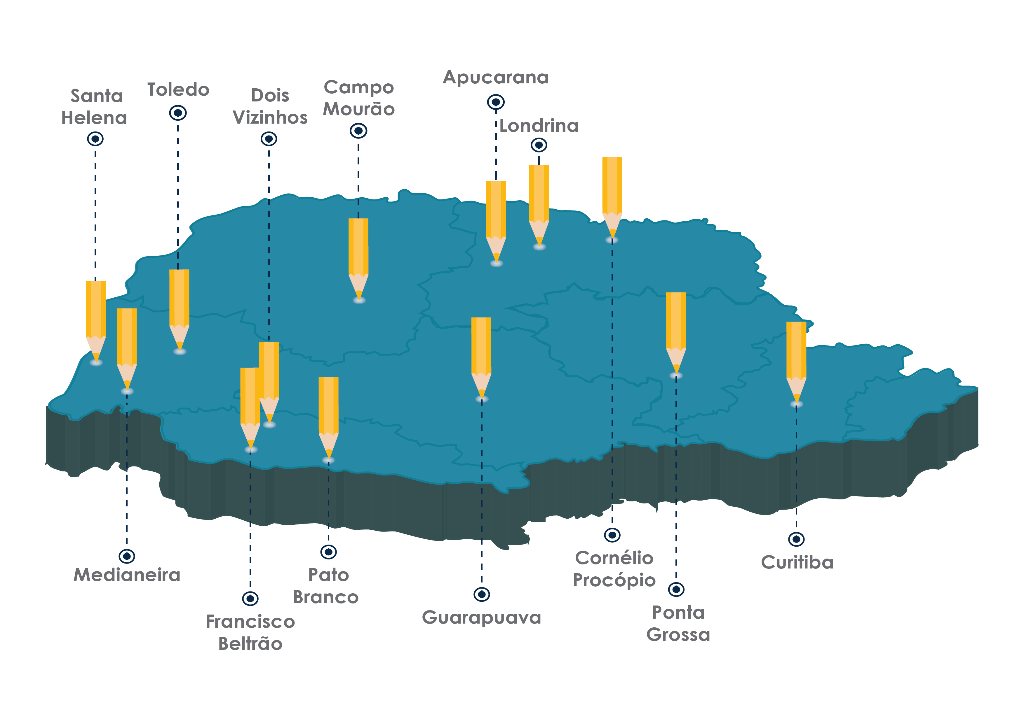
\includegraphics[height = \dimen1]{fig-campi-map}}
			\usebox0%
			\llap{%
				\raisebox{\ht0-\height}{%
					\href{https://www.utfpr.edu.br/campus}{%
						
\includegraphics[height = 10mm]{fig-campi-map-qr-code}%
					}%
				}%
			}
			\SourceOrNote{\textcite{UTFPR2017}}
		\end{figure}
		
		\column{0.5\textwidth-0.5\columnsep}
		
		É possível clicar na Fig.~\ref{fig:flow-experiment-photo} para reproduzir um vídeo dependendo do visualizador de PDF\@.
		
		\begin{figure}[!htb]
			\caption{Experimento de mecânica dos fluidos}%
			\label{fig:flow-experiment-photo}
			\only<presentation>{\dimen1 = 28mm}%% Apresentação: tamanho de figura
			\only<article>{\dimen1 = 48mm}%% Artigo: tamanho de figura
			\movie[showcontrols = true]{%
				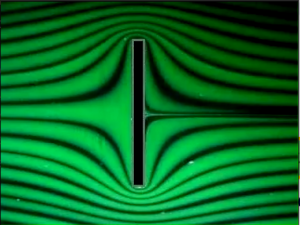
\includegraphics[height = \dimen1]{./Multimedia/flow-experiment-photo}%
			}{./Multimedia/flow-experiment.flv}
			\SourceOrNote{autoria própria (\YearNum)}
		\end{figure}
		
		\begin{exampleblock}{\faExternalLinkSquare*\ Exemplos de atalhos para vídeos (ou outros arquivos)}
			
			\begin{itemize}
				\item[\tiny\faFileVideo] \href{run:./Multimedia/flow-experiment.flv}{Experimento de mecânica dos fluidos (arquivo de vídeo).}
				\item[\tiny\faFileVideo] \href{https://youtu.be/6UlsArvbTeo?si=aU2mbh-XGX3o6nWe}{Escoamento sobre aerofólios (vídeo \ENLang{online}).}
			\end{itemize}
			
		\end{exampleblock}
		
	\end{columns}
	
\end{frame}

\subsection{Gráficos e tabelas}

\begin{frame}
	
	\only<presentation>{\vspace*{-\bigskipamount}}%% Apresentação: espaçamento
	
	\begin{columns}[t]
		
		\column{0.5\textwidth-0.5\columnsep}
		
		A Figura~\ref{fig:t-x}\footnote{Gráfico produzido no ambiente \LaTeX\ \texttt{tikzpicture} do pacote \LaTeX\ \texttt{tikz} a partir do arquivo \texttt{grph-t-x.tex} em \texttt{./Figures/}.} foi inserida usando o ambiente \LaTeX\ \texttt{figure} e numerada automaticamente.
		
		\begin{figure}[!htb]
			\caption{Exemplo de legenda de figura}%
			\label{fig:t-x}
			\only<presentation>{\dimen1 = 36mm}%% Apresentação: tamanho de figura
			\only<article>{\dimen1 = 56mm}%% Artigo: tamanho de figura
			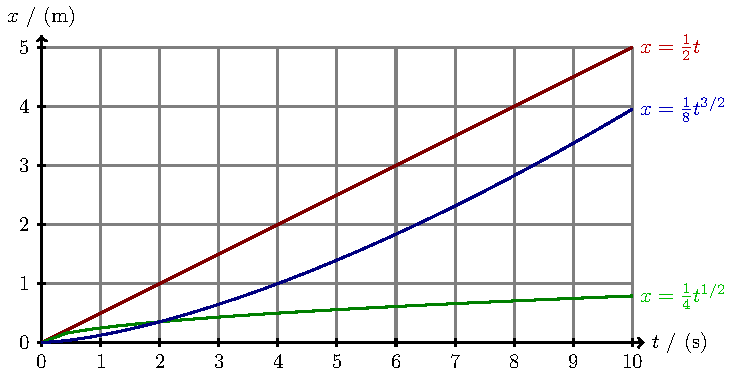
\includegraphics[height = \dimen1]{grph-t-x}
			\SourceOrNote{autoria própria (\YearNum)}
		\end{figure}
		
		\column{0.5\textwidth-0.5\columnsep}
		
		A Tabela~\ref{tab:L-dimensions} foi inserida usando o ambiente \LaTeX\ \texttt{table} e numerada automaticamente.
		
		\begin{table}[!htb]
			\caption{Exemplo de legenda de tabela}%
			\label{tab:L-dimensions}
			\begin{tabularx}{\linewidth}{@{}lYYYY@{}}
				\toprule%
				\multicolumn{1}{@{}c}{\textbf{Caso}} &
				$\MathBF{L / \Unit{(m)}}$            &
				$\MathBF{L^2 / \Unit{(m^2)}}$        &
				$\MathBF{L^3 / \Unit{(m^3)}}$        &
				$\MathBF{L^4 / \Unit{(m^4)}}$        \\ \midrule%
				A & 1 & 1  & 1   & 1   \\
				B & 2 & 4  & 8   & 16  \\
				C & 3 & 9  & 27  & 81  \\
				D & 4 & 16 & 64  & 256 \\
				E & 5 & 25 & 125 & 625 \\ \bottomrule%
				\addlinespace[\belowcaptionskip]
			\end{tabularx}
			\SourceOrNote{autoria própria (\YearNum)}
		\end{table}
		
		\begin{alertblock}{\faInfoCircle\ Ferramentas para gerar ou editar tabelas em \LaTeX}
			
			\begin{itemize}
				\selectlanguage{english}
				\item[\tiny\faTools] \href{https://www.tablesgenerator.com/}{Tables Generator\LinkIcon}.
				\item[\tiny\faTools] \href{https://www.latex-tables.com/}{\LaTeX\ Tables Editor\LinkIcon}.
			\end{itemize}
			
		\end{alertblock}
		
	\end{columns}
	
\end{frame}


\section{Conclusões}%
\label{sect:concl}
%\input{modules/module5}

\begin{frame}

As conclusões ou considerações finais podem ser apresentadas como uma lista de itens, enfatizando as contribuições do trabalho:

\begin{itemize}
\item Primeiro item de conclusão.
\item Segundo item de conclusão.
\item Terceiro item de conclusão.
\item Quarto item de conclusão.
\item Quinto item de conclusão.
\end{itemize}

\end{frame}

\section<presentation>{\refname}%% Apresentação: Referências (seção e rótulo)
\label<presentation>{sect:ref}

\only<presentation>{\frame[allowframebreaks]{\printbibliography[heading = none]}}%% Apresentação: Referências

\section{Agradecimentos}%
\label{sect:ack}

\RespNotice[Declaração de Responsabilidade]{O{(s)} autor{(es)} é{(são)} o{(s)} único{(s)} responsável{(eis)} pelas informações contidas neste documento.}

\begin{frame}

\dimen1 = 10mm%

\pause%

\begin{itemize}
\only<presentation>{%% Apresentação: Agradecimentos (aos participantes)
  \item<+->[\scriptsize\faUsers] Aos participantes:%
  \begin{itemize}%
  \item Por suas questões, seus comentários e sua atenção.%
  \ufootnote{\RespNoticeFull}%% Declaração de Responsabilidade
  \end{itemize}%
}
\item<+->[\scriptsize\faUniversity] Às instituições:
\begin{itemize}
\item Pelo apoio recebido para o desenvolvimento deste trabalho e a participação neste evento:\par%
\begin{minipage}[c][20mm]{\linewidth}
\Logo[height = \dimen1]{capes-l}%
\hfill%
\Logo[height = \dimen1]{cnpq-l}%
\hfill%
\Logo[height = \dimen1]{fa-l}%
\hfill%
\Logo[height = \dimen1]{Extra}%
\hfill%
\Logo[height = \dimen1]{public-education-l}%
\hspace*{0.2\dimen1}%
\Logo[height = \dimen1]{utfpr-l}
\end{minipage}
\end{itemize}
\end{itemize}

\begin{columns}[t]

\column{0.9\textwidth-0.5\columnsep}

\begin{exampleblock}<presentation|+->{\faTalking\ Palestrante}%% Apresentação: Palestrante

\begin{minipage}{0.75\dimen1}
\color{UTFPRYellow}
\setkeys{draftfigure}{content = {\faUserTie\\Inserir\\Foto}, size = {tiny}}
\includegraphics[width = 0.75\dimen1, height = \dimen1, draft]{example-image}
\end{minipage}%
\hfill%
\begin{minipage}{\linewidth-1em-0.75\dimen1}
\InfoList{\faUserTie}{Nome Completo do{(a)} Autor{(a)}}\par%
\InfoList{\faUniversity}{\UTFPRName}\par%
\InfoList{\faEnvelope}{\email{author1@domain}}
\end{minipage}

\end{exampleblock}

\column{0.1\textwidth-0.5\columnsep}

\begin{alertblock}<presentation|+->{\faPlus\ \faInfoCircle}%% Apresentação: Mais Informações

\centering%
\href{https://www.utfpr.edu.br/}{
\includegraphics[height = \dimen1]{utfpr-qr-code}}

\end{alertblock}

\end{columns}

\end{frame}

\only<article>{\printbibliography}%% Artigo: Referências

\section<article>{\RespNoticeTitle}%% Artigo: Declaração de Responsabilidade (seção e rótulo)
\label<article>{sect:resp-not}

\only<article>{\RespNoticeText}%% Artigo: Declaração de Responsabilidade

%% Fim do documento
\end{document}
